%%%%%%%%%%%%%%%%%%%%%%%%%%%%%%%%%%%%%%%%%
% Jacobs Landscape Poster
% LaTeX Template
% Version 1.1 (14/06/14)
%
% Created by:
% Computational Physics and Biophysics Group, Jacobs University
% https://teamwork.jacobs-university.de:8443/confluence/display/CoPandBiG/LaTeX+Poster
% 
% Further modified by:
% Nathaniel Johnston (nathaniel@njohnston.ca)
%
% This template has been downloaded from:
% http://www.LaTeXTemplates.com
%
% License:
% CC BY-NC-SA 3.0 (http://creativecommons.org/licenses/by-nc-sa/3.0/)
%
%%%%%%%%%%%%%%%%%%%%%%%%%%%%%%%%%%%%%%%%%

%----------------------------------------------------------------------------------------
%	PACKAGES AND OTHER DOCUMENT CONFIGURATIONS
%----------------------------------------------------------------------------------------

\documentclass[final]{beamer}

\usepackage[scale=1.24]{beamerposter} % Use the beamerposter package for laying out the poster

\usetheme{confposter} % Use the confposter theme supplied with this template


\definecolor{cpurple}{Gray}{0.15}
\definecolor{corange}{RGB}{246,103,51}

\setbeamercolor{block title}{fg=ngreen,bg=white} % Colors of the block titles
\setbeamercolor{block body}{fg=black,bg=white} % Colors of the body of blocks
\setbeamercolor{block alerted title}{fg=Gray!15,bg=BrickRed!95} % Change the alert block title colors
\setbeamercolor{block alerted body}{fg=black,bg=BrickRed!05} % Change the alert block body colors
% Many more colors are available for use in beamerthemeconfposter.sty

\setbeamercolor{background canvas}{bg=gray!50}

%-----------------------------------------------------------
% Define the column widths and overall poster size
% To set effective sepwid, onecolwid and twocolwid values, first choose how many columns you want and how much separation you want between columns
% In this template, the separation width chosen is 0.024 of the paper width and a 4-column layout
% onecolwid should therefore be (1-(# of columns+1)*sepwid)/# of columns e.g. (1-(4+1)*0.024)/4 = 0.22
% Set twocolwid to be (2*onecolwid)+sepwid = 0.464
% Set threecolwid to be (3*onecolwid)+2*sepwid = 0.708

\newlength{\sepwid}
\newlength{\onecolwid}
\newlength{\twocolwid}
\newlength{\threecolwid}
\setlength{\paperwidth}{48in} % A0 width: 46.8in
\setlength{\paperheight}{36in} % A0 height: 33.1in
\setlength{\sepwid}{0.024\paperwidth} % Separation width (white space) between columns
\setlength{\onecolwid}{0.22\paperwidth} % Width of one column
\setlength{\twocolwid}{0.464\paperwidth} % Width of two columns
\setlength{\threecolwid}{0.708\paperwidth} % Width of three columns
\setlength{\topmargin}{-0.5in} % Reduce the top margin size
%-----------------------------------------------------------

\usepackage{graphicx}  % Required for including images

\usepackage{booktabs} % Top and bottom rules for tables

\usepackage{amsmath}

%----------------------------------------------------------------------------------------
%	TITLE SECTION 
%----------------------------------------------------------------------------------------

\title{\huge Computer model calibration for design, with an application to wind turbine blades} % Poster title

\author{Carl Ehrett\textsuperscript{1,2}, Andrew Brown\textsuperscript{1,2}, Sez Atamturktur\textsuperscript{1,3}, Christopher Kitchens\textsuperscript{1,4}, Mingzhe Jiang\textsuperscript{1,4}, Caleb Arp\textsuperscript{1,4}, Evan Chodora\textsuperscript{1,3}} % Author(s)

\institute{\textsuperscript{1}Clemson University, \textsuperscript{2}Department of Mathematical Sciences, \textsuperscript{3}Glenn Department of Civil Engineering, 
\textsuperscript{4}Chemical and Biomolecular Engineering} % Institution(s)

%----------------------------------------------------------------------------------------

\begin{document}


\addtobeamertemplate{alertblock end}{}{\vspace*{1ex}} % White space under blocks
\addtobeamertemplate{alertblock alerted end}{}{\vspace*{2ex}} % White space under highlighted (alert) blocks

\setlength{\belowcaptionskip}{1ex} % White space under figures
\setlength\belowdisplayshortskip{2ex} % White space under equations



\begin{frame}[t] % The whole poster is enclosed in one beamer frame

\vspace{-20mm}

\begin{columns}[t] % The whole poster consists of three major columns, the second of which is split into two columns twice - the [t] option aligns each column's content to the top

\begin{column}{\sepwid}\end{column} % Empty spacer column

\begin{column}{\onecolwid} % The first column

%----------------------------------------------------------------------------------------
%	OBJECTIVES
%----------------------------------------------------------------------------------------

%----------------------------------------------------------------------------------------
%	INTRODUCTION
%----------------------------------------------------------------------------------------

\begin{alertblock}{Computer model calibration}
\begin{itemize}
\item Researchers increasingly look to computer experiments to investigate phenomena where physical experimentation is difficult or impossible\cite{Sacks1989,Santner2003a}.
\item Computer models may include unknown inputs (calibration inputs) that must be estimated\cite{Kennedy2001}. 

%\item E.g.: a model's output depends upon a physical constant which is unknown. 

\item Calibration input is often estimated by combining simulator output with field data. 

\item Calibration is ordinarily thought of as bringing a computer model into agreement with reality.
%\item Previous explorations of computer model calibration have approached calibration as a matter of bringing a computer model into agreement with physical reality.

\end{itemize}

\end{alertblock}

%------------------------------------------------

\begin{alertblock}{Full model}

Where $\boldsymbol \theta$ is the vector of true (optimal) values of the calibration parameter, $\mathbf w$ is a vector of control parameter settings, and $\boldsymbol \epsilon\sim N_3(0,\mathrm{diag}(\sigma^2_d,\sigma^2_r,\sigma^2_c))$, we may describe the model for the desired data as
\[
f(\mathbf w,\boldsymbol \theta) = f(\mathbf w) = \eta(\mathbf w,\boldsymbol \theta) + \boldsymbol \epsilon
\]
Note that we are here assuming that the original simulator $\eta(\cdot,\boldsymbol\theta)$ is unbiased with respect to $f$ when the true values of $\boldsymbol\theta$ are used as inputs.

\end{alertblock} 

%---------------------------------------------------


\begin{alertblock}{Finite element smulator}
We rely on a finite element simulator of the blade cost and performance.

\begin{figure}[h!]
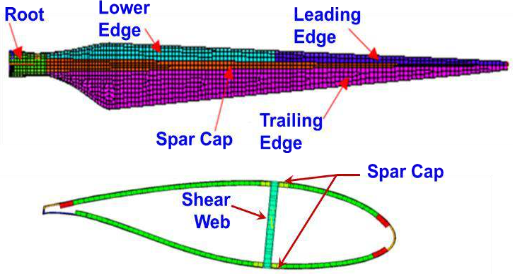
\includegraphics[width=0.6\linewidth]{blade3}
%\caption{Wind turbine blade}
\label{blade}
\end{figure}

\vspace{-18mm}
\begin{itemize}
\item Calibration inputs: volume fraction, thickness of blade material. Control input: temperature.

%\item Control input is temperature.

\item Outputs are tip deflection, rotation, and cost; the design goal is to minimize these.

\item Model utilizes \texttt{ANSYS} simulation software; computation cost is too high for use in MCMC.

%\item \texttt{ANSYS} model cost too high for use in MCMC.

\end{itemize}
\end{alertblock}




%------------------------------------------------

%\begin{alertblock}{Central idea}
%\begin{itemize}
%\item Previous explorations of computer model calibration have approached calibration as a matter of bringing a computer model into agreement with physical reality.
%
%\item In the present work, we consider computer model calibration as a method for design. 
%
%\item Under this framework, we calibrate a computer model not using physical experimental data, but rather using ``desired data'' which describes the performance one hopes to achieve in the simulated system. 
%
%\end{itemize}
%
%\end{alertblock} 

%----------------------------------------------------------------------------------------

\end{column} % End of the first column



\begin{column}{\sepwid}\end{column} % Empty spacer column

\begin{column}{\twocolwid} % Begin a column which is two columns wide (column 2)

\setbeamercolor{block alerted title}{fg=Gray!15,bg=MidnightBlue!95} % Change the alert block title colors
\setbeamercolor{block alerted body}{fg=black,bg=MidnightBlue!10} % Change the alert block body colors

\begin{alertblock}{Central idea}

Previous explorations of computer model calibration have approached calibration as a matter of bringing a computer model into agreement with physical reality\cite{Bayarri2007,Kennedy2001,Higdon2004,Williams2006}. \textbf{In the present work, we consider computer model calibration as a method for design.} Under this framework, we calibrate a computer model not using physical experimental data, but rather using ``desired data'' which describes the performance one hopes to achieve in the simulated system. 

\end{alertblock} 

\setbeamercolor{block alerted title}{fg=Gray!15,bg=BrickRed!95} % Change the alert block title colors
\setbeamercolor{block alerted body}{fg=black,bg=BrickRed!05} % Change the alert block body colors

\begin{columns}[t,totalwidth=\twocolwid] % Split up the two columns wide column

\begin{column}{\onecolwid}\vspace{-.6in} % The first column within column 2 (column 2.1)

%----------------------------------------------------------------------------------------
%	MATERIALS
%----------------------------------------------------------------------------------------

\begin{alertblock}{Gaussian process emulator}

Gaussian processes (GPs) can be thought of as random functions which are generalizations of multivariate normal random variables\cite{OHagan1978}. A GP is fully characterized by its mean function $\mu:D\to R$ and covariance function $V:D\times D\to R$, where $D$ is the domain of the process.

\begin{figure}[h!]
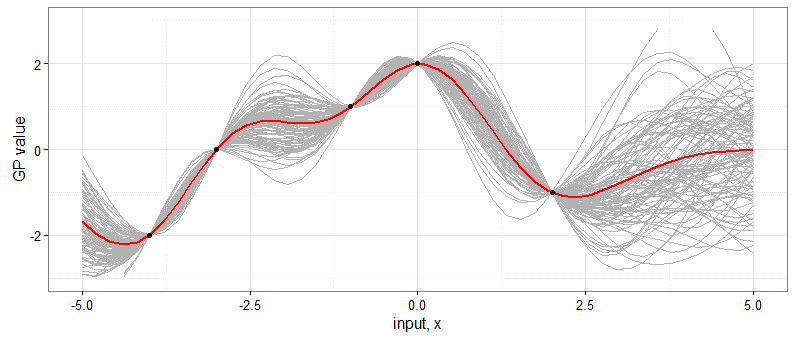
\includegraphics[width=0.95\linewidth]{../../gp_example}
\caption{Example of a univariate Gaussian process}
\label{gp_ex}
\end{figure}



GPs are advantageous for emulating computationally expensive deterministic computer code\cite{Sacks1989,Santner2003a} because 
%\vspace{-8mm}
\begin{itemize}
\item Use of a GP does not require detailed foreknowledge of the approximate parametric form of the model; we often lack such knowledge
\item GPs easily interpolate the observed data; since the simulation code is deterministic and free of observation error, this is desirable
\item The variance of GPs provides a natural form of uncertainty quantification (see Figure \ref{gp_ex})
\end{itemize}



\end{alertblock}


%----------------------------------------------------------------------------------------

\end{column} % End of column 2.1

\begin{column}{\onecolwid}\vspace{-.6in} % The second column within column 2 (column 2.2)

%----------------------------------------------------------------------------------------
%	METHODS
%----------------------------------------------------------------------------------------

\begin{alertblock}{Emulator implementation}

Model inputs are a dummy input $x_1$ (to convert trivariate output into univariate), temperature $x_2$, volume fraction $x_3$ and thickness $x_4$. For our GP emulator prior we use the covariance function
\[
V(\mathbf x,\mathbf x' ) = \frac1\lambda \exp\{-\sum_{i=1}^4 \beta_i(x_i-x_i')^2 \}
\]
where $\lambda,\boldsymbol \beta$ were estimated using gradient methods to find their MLEs. 
% Ref, + more expl?
A prior mean $\mu(\mathbf x) = 0$ was also used. Observations $\eta(\mathbf x_i)$, $i=1,\cdots,504$ were collected from the simulation model using a LHC design. %ref?
The updated (posterior) GP emulator has mean given by
\[\mu^*(\mathbf x) = v(\mathbf x)^T \Sigma^{-1} \boldsymbol \eta \]
where $v(\mathbf x) = (V(\mathbf x, \mathbf x_1),\cdots,V(\mathbf x,\mathbf x_{504}))^T$, $\Sigma$ is a matrix with $\Sigma_{i,j} = V(\mathbf x_i,\mathbf x_j)$, and $\boldsymbol \eta = (\eta(\mathbf x_1),\cdots,\eta(\mathbf x_{504}))^T$. The updated covariance:
\[
V^* (\mathbf x, \mathbf x') = V(\mathbf x, \mathbf x') - v(\mathbf x)^T \Sigma^{-1} v(\mathbf x')
\]
\end{alertblock}

%----------------------------------------------------------------------------------------

\begin{alertblock}{Desired data}

We calibrate the model to ``desired data'' which reflect extremely low tip deflection, rotation, and cost. Because we are antecedently ignorant of how close the model can come to our desired data, we place an improper $1/\sigma^2$ prior on the observation variance of each model output. We considered a range of desired outcomes.

\end{alertblock}

\end{column} % End of column 2.2

\end{columns} % End of the split of column 2 - any content after this will now take up 2 columns width

%----------------------------------------------------------------------------------------
%	IMPORTANT RESULT
%----------------------------------------------------------------------------------------

\setbeamercolor{block alerted title}{fg=Gray!15,bg=MidnightBlue!95} % Change the alert block title colors
\setbeamercolor{block alerted body}{fg=black,bg=MidnightBlue!10} % Change the alert block body colors



\setbeamercolor{block alerted title}{fg=Gray!15,bg=BrickRed!95} % Change the alert block title colors
\setbeamercolor{block alerted body}{fg=black,bg=BrickRed!05} % Change the alert block body colors


%----------------------------------------------------------------------------------------

\begin{columns}[t,totalwidth=\twocolwid] % Split up the two columns wide column again

\begin{column}{\onecolwid} % The second column within column 2 (column 2.2)

%----------------------------------------------------------------------------------------
%	RESULTS
%----------------------------------------------------------------------------------------
%
%\begin{alertblock}{Results}
%
%\begin{figure}
%
\includegraphics[width=0.8\linewidth]{placeholder.jpg}
%\caption{Figure caption}
%\end{figure}
%
%Nunc tempus venenatis facilisis. Curabitur suscipit consequat eros non porttitor. Sed a massa dolor, id ornare enim:
%
%\begin{table}
%\vspace{2ex}
%\begin{tabular}{l l l}
%\toprule
%\textbf{Treatments} & \textbf{Response 1} & \textbf{Response 2}\\
%\midrule
%Treatment 1 & 0.0003262 & 0.562 \\
%Treatment 2 & 0.0015681 & 0.910 \\
%Treatment 3 & 0.0009271 & 0.296 \\
%\bottomrule
%\end{tabular}
%\caption{Table caption}
%\end{table}
%
%\end{alertblock}

%----------------------------------------------------------------------------------------

\end{column} % End of column 2.2

\end{columns} % End of the split of column 2

\end{column} % End of the second column

\begin{column}{\sepwid}\end{column} % Empty spacer column

\begin{column}{\onecolwid} % The third column

%----------------------------------------------------------------------------------------
%	CONCLUSION
%----------------------------------------------------------------------------------------

\begin{alertblock}{MCMC implementation}

\begin{itemize}

\item Calibrate volume fraction and thickness to the desired data. Set a uniform prior over each.

\item Each iteration of the MCMC, draw new values for $x_3,x_4$, and the observation variances.% for each of tip deflection, rotation, and cost $(\sigma^2_{d},\sigma^2_{r},\sigma^2_{c}$). 

\item Where $\mathbf y$ is the desired data, $\mathcal D = (\mathbf y,\boldsymbol \eta)^T$ and $\Sigma_{\mathcal D} = \mathrm {Var}(\mathcal D)$, the likelihood of $\mathcal D$ is
\[%\begin{multline*}
L(\mathcal D| x_3,\!x_4,\!\lambda,\!\boldsymbol \beta,\!\Sigma_{\mathcal D}) = 
|\Sigma_{\mathcal D} | ^{-\frac 12} \exp \{\! -\frac 12 \mathcal D ^T \Sigma_{\mathcal D}^{-1} \mathcal D  \}
\]%\end{multline*}
hence\cite{Williams2006} the full posterior density is:
\begin{flalign*}
\pi(x_3,x_4,\sigma^2_d,\sigma^2_r,\sigma^2_c) \propto  & \frac{L(\mathcal D| x_3,\!x_4,\!\lambda,\!\boldsymbol \beta,\!\Sigma_{\mathcal D})}{\sigma^2_d\sigma^2_r\sigma^2_c}
\end{flalign*}
%
%\vspace{-20mm}
%\begin{eqnarray*}
%%\phantom = &L(\mathcal D| x_3,\!x_4,\!\lambda,\!\boldsymbol \beta,\!\Sigma_{\mathcal D}) \times &
%%\pi(x_3)\times \pi(x_4) \times \\&& \pi(\sigma^2_d) \times \pi (\sigma^2_r) \times \pi(\sigma^2_c)\\
%=&L(\mathcal D| x_3,\!x_4,\!\lambda,\!\boldsymbol \beta,\!\Sigma_{\mathcal D}) \times& \frac1{\sigma^2_d\sigma^2_r\sigma^2_c}
%\end{eqnarray*}


\item Eliminate boundary constraints: $z_i = \mathrm{logit}(x_i)$, $\tau_j = \log(\sigma^2_j)$ for $i=3,4$, $j=d,r,c$.

\item We use the Metropolis-Hastings %ref
algorithm\cite{Hastings1970}; we set normal proposals on $z_i^{(n)}|z_i^{(n-1)}$ and $\tau_j^{(n)}|\tau_j^{(n-1)}$, $\forall i \forall j$.

\item In burn-in, the proposal distribution adapts using the sample covariance of previous draws, achieving optimal acceptance ratios ($\sim40\%$).

\end{itemize}



\end{alertblock}

%----------------------------------------------------------------------------------------
%	ADDITIONAL INFORMATION
%----------------------------------------------------------------------------------------

\begin{alertblock}{Results}


\begin{figure}[h!]
%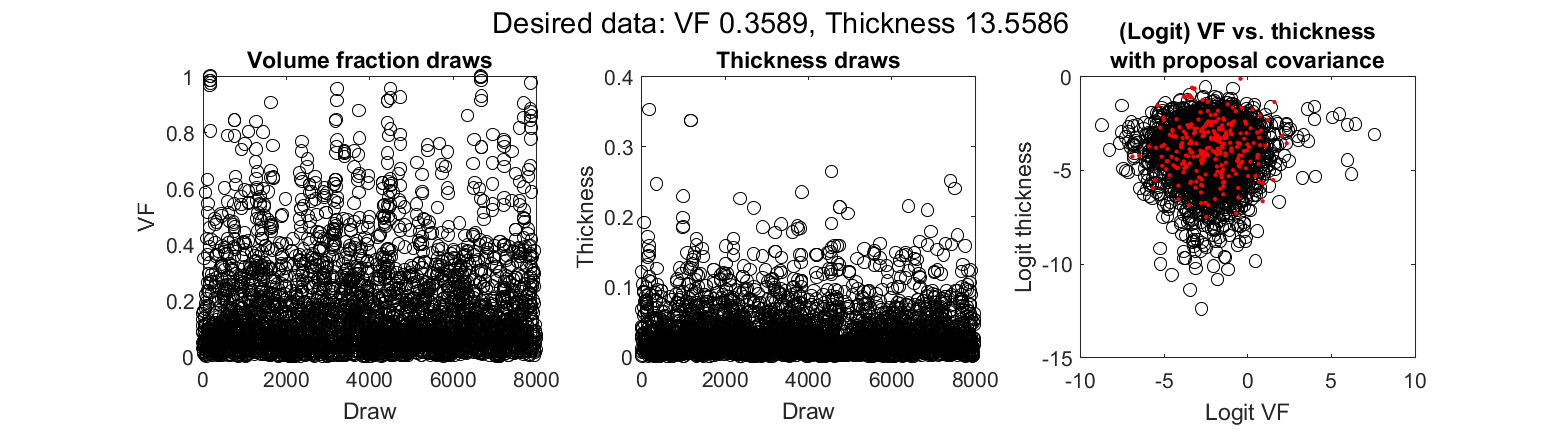
\includegraphics[width=\linewidth]{FIG1}
%\caption{}
\label{res}
\end{figure}

\vspace{-24mm}
\begin{itemize}
\item Posterior means are sensitive to choice of desired data. Therefore it is advisable to consider a surface over a range of desired data.
\item Where desired output is insufficiently ambitious, the MCMC output reflects this as a lack of identifiability in the calibration inputs.
\end{itemize}

\vspace{-4mm}
\begin{figure}[h!]
%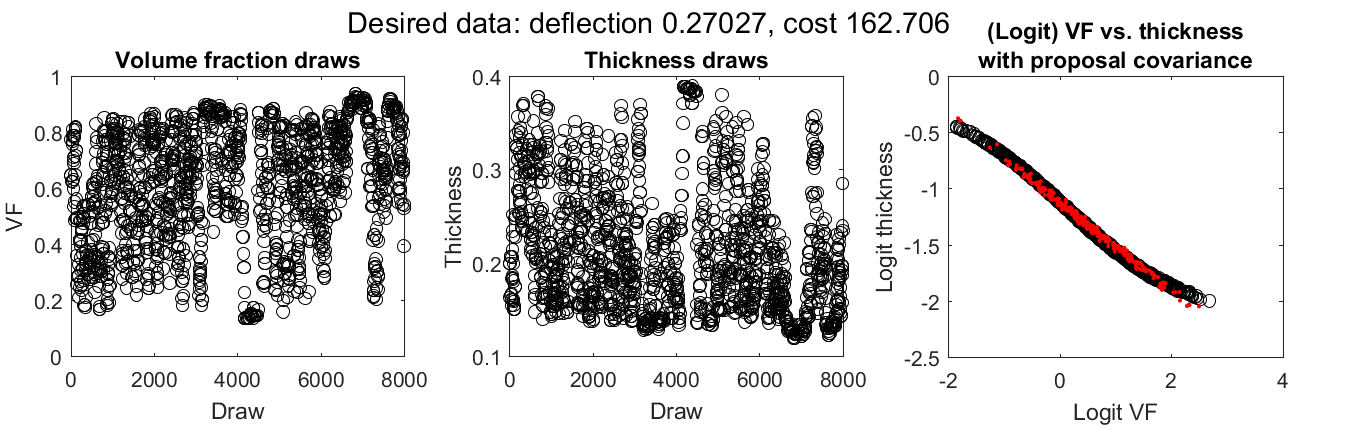
\includegraphics[width=\linewidth]{FIG2}
%\caption{}
\label{unident}
\end{figure}

\vspace{-20mm}
\end{alertblock}

%----------------------------------------------------------------------------------------
%	REFERENCES
%----------------------------------------------------------------------------------------

%\begin{alertblock}{References}
%
%\nocite{*} % Insert publications even if they are not cited in the poster
%\small{\bibliographystyle{unsrt}
%\bibliography{sample}\vspace{0.75in}}
%
%\end{alertblock}

%----------------------------------------------------------------------------------------
%	ACKNOWLEDGEMENTS
%----------------------------------------------------------------------------------------

%\setbeamercolor{alertblock title}{fg=red,bg=white} % Change the block title color
%
%\begin{alertblock}{Acknowledgements}
%
%\small{\rmfamily{Nam mollis tristique neque eu luctus. Suspendisse rutrum congue nisi sed convallis. Aenean id neque dolor. Pellentesque habitant morbi tristique senectus et netus et malesuada fames ac turpis egestas.}} \\
%
%\end{alertblock}

\begin{alertblock}{References}
{
\tiny

\bibliographystyle{ieeetr}

\bibliography{poster}
}

\end{alertblock}

%----------------------------------------------------------------------------------------
%	CONTACT INFORMATION
%----------------------------------------------------------------------------------------

\setbeamercolor{alertblock alerted title}{fg=black,bg=norange} % Change the alert block title colors
\setbeamercolor{alertblock alerted body}{fg=black,bg=white} % Change the alert block body colors

\begin{alertblock}{Contact Information}

%\begin{itemize}
%\item Web: \href{http://www.university.edu/smithlab}{http://www.university.edu/smithlab}
%\item Email: \href{mailto:cehrett@clemson.edu}{cehrett@clemson.edu}
%\vspace{-15mm}
\centering Carl Ehrett\\
\centering Email: \href{mailto:cehrett@clemson.edu}{cehrett@clemson.edu}
%\item Phone: +1 (774) 234 7388
%\end{itemize}

%\vspace{-10mm}
\end{alertblock}


%----------------------------------------------------------------------------------------

\end{column} % End of the third column

\end{columns} % End of all the columns in the poster

\end{frame} % End of the enclosing frame

\end{document}
